%   This is a template for a senoir honours project report.
\documentclass[A4sheet,12pt]{article}
\usepackage{fullpage}
\usepackage[pdftex]{graphicx}
\usepackage{amsmath}
\usepackage{float}
\usepackage{textgreek}
\usepackage{listings}
\setlength{\parindent}{0pt}
\usepackage[a4paper,left=1.25cm, right=1.25cm, top=1.5cm, bottom=2cm]{geometry}
\usepackage{hyperref}


%
%                       This section generates a title page
%                       Edit only the sections indicated to put
%                       in the project title, your name, supervisor,
%                       project length in weeks and submission date
%
\begin{document}
\pagestyle{empty}                       % No numbers on title page      

\par\noindent
\includegraphics[width=12cm]{figures/PandA_crest.pdf}

\par\noindent                                           % Centre Title, and name
\vspace*{2cm}
\begin{center}
        \Large\bf \Large\bf Data Acquisition and Handling Project\\
        \LARGE\bf Making Accurate Measurements of Particle Masses
\end{center}
\vspace*{0.5cm}
\begin{center}
        \bf Achille Quarante, Matthew Kerr \\
        November 2022                            
\end{center}
\vspace*{5mm}
%
%                       Insert your abstract HERE                
\begin{abstract}
        LHCb data on the invariant mass of $\Upsilon$ mesons from high energy $PP$ collisions was analysed in this project. Various models were fitted to the data and analysed, and uncertainties were calculated for each of these. The accuracy of these fits were also calculated and compared against each other, determining that the best fit is the double Gaussian. This was then used to determine values for the the three $\Upsilon$ mesons masses to be 9.4(3), 10.0(3) and 10.3(3) $[GeV/c^2]$, along with uncertainties in these values from both statistical and systematic errors.
\end{abstract}

\vspace*{1cm}


\vfill            

\newpage
%
%                       End of Title Page
\pagestyle{plain}                               % Page numbers at bottom
\setcounter{page}{1}                            % Set page number to 1
\tableofcontents                                % Makes Table of Contents

\clearpage

\addcontentsline{toc}{section}{Introduction and Background}
\section*{Introduction and Background}
The data used in this research project is based on the 2013 paper by the LHCb Team titled"Production of J/$\psi$ and $\Upsilon$ mesons in pp collisions at $\sqrt{\text{s}}$ = 8 TeV"\cite{origpaper}. The aim of this paper was to study the production of J/$\psi$ and $\Upsilon$ mesons after a pp (proton-proton) collision at $\sqrt{\text{s}}$ = 8 TeV (total center of mass collision energy) in the LHC. The data used in this paper was gathered in April 2012. In this research project, we focused on analysing the $\Upsilon$ data with main objective of determining the invariant mass of the muon pairs.\\

Analysis of the quality of fits was done by taking the reduced $\chi ^2$, which is defined as such,

\begin{equation}
    \chi ^2 = \frac{1}{\nu} \sum_i \frac{(O_i - F_i)^2}{\sigma_{i}^{2} }
\end{equation}

Where $\nu$ is the number of data points used minus the number of parameters used in the fit. $O_i$ is a data point at $i$, $F_i$ is the value of the fit at point $i$ and $\sigma_i$ is the standard deviation.




\addcontentsline{toc}{section}{Methods}
\section*{Methods}
\addcontentsline{toc}{subsection}{Cleaning the Data}
\subsection*{Cleaning the Data}

A few attempts at removing background noise from the data were made. Heat maps of rapidity, transverse momentum of the muon pair, and the transverse momentum of each of the individual muons against the invariant mass were plotted. Some examples of these are shown below.

\begin{figure}[H]
\centering
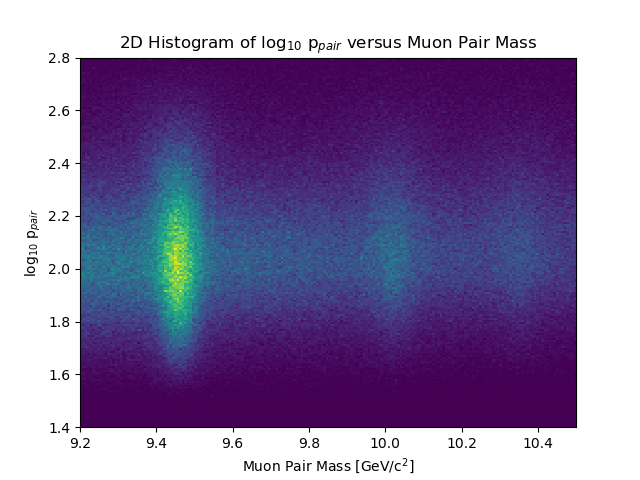
\includegraphics[width=0.48\columnwidth]{figures/log_mom_pair_xmass_2d_hist.png}
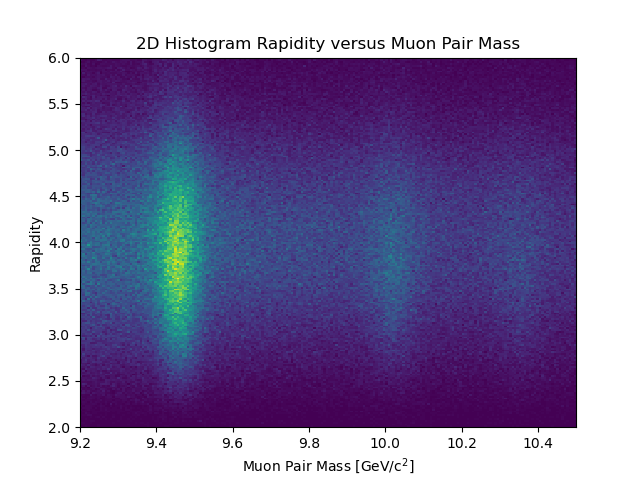
\includegraphics[width=0.48\columnwidth]{figures/rap_xmass_2d_hist.png}
\caption{2D histograms of the the transverse momentum and rapidity against the invariant pair mass. These were used to try and clean the data by neglecting terms outside of the center regions of the Y-axis.}
\label{fig:2d_hists_ex}
\end{figure}

Cutoff lines parallel to the x-axis, above and below the main signal regions were set, in an attempt to isolate the signals that came from muon decays. To measure whether the signals from the decays had been isolated, the ratios of the decrease in the signal across the background region and the peak region was measured and compared. If these ratios are equal, then the decay signals hadn't been isolated, as an even number of signals had been taken from the background and the peak region. However, if this ratio of the peak region was smaller than the background, then more data has been taken from the background regions than the peaks, and the decay signals had be isolated, cleaning the data. \\

One additional heat map was constructed. This map concerned a value that we named R.

\begin{equation}
    R = \frac{\lvert p_{t, 1} - p_{t, 2}\rvert}{p_{t, 1} + p_{t, 2}}
\end{equation}

The theory behind this value, was that in the production of the $\Upsilon$ mesons, the resultant muons that are produced will have to have equal and opposite momenta in the transverse direction(as the initial transverse momentum is 0). Therefore, if a signal came from a meson decay, taking the difference between the modulus of these values should result in a value of 0(within a range of uncertainty). However, the difference between some of the very fast muons may end up being quite large due to the large uncertainties in the measurements. This problem was dealt with by normalising the value of R by the sums of the transverse momenta.\\

If a measurement was from background muons, then the likelihood them having equal and opposite momenta in the transverse direction is low. This means that in theory, neglecting any muon measurements with a large value of R, should isolate measurements from the meson decays and clean the data. \\

The data was also binned to try and remove some noise. This was done by using the Freedman–Diaconis rule to determine the width of the bins. This method is designed to minimize the integral of the squared difference between the heights of the bins in a histogram\cite{freedman} and is calculated as follows:

\begin{equation}
    W = 2\frac{IQR(x)}{\sqrt[3]{n}}
\end{equation}

Where $IQR(x)$ is the interquartile range of the data and $n$ is the number of data points. Different models were then fitted to this data using the Negative Log Likelihood method defined below:
\begin{equation}
    NLL = - \sum_{i} P(t_i|\tau_{\mu})
\end{equation}
Where $t_i$ is an observable quantity depending on parameter $\tau_{\mu}$. The value of $\tau_{\mu}$ is optimised by minimising $NLL$
\addcontentsline{toc}{subsection}{Exponential Background Fit}
\subsection*{Exponential Background Fit}

The background was estimated to decay exponentially, so to fit this to the data, regions in the invariant mass where the counts where estimated to be purely background were isolated and an exponential function can be fit to the data from these regions using SciPy's \verb|optimize.curve_fit()| function. 

\begin{equation}
    f(x) = A\cdot e^{\delta + c\cdot x}
\end{equation}

Where $A$, $\delta$ and $c$ are free parameters that are allowed to fit and $x$ is the independent variable. 

\addcontentsline{toc}{subsection}{Gaussian Fit}
\subsection*{Gaussian Fit}

The simplest model fitted to the peaks was a Gaussian function. This was done by constructing a Probability Density Function made of three Gaussian's and an exponential decay. The equation of the Gaussian model can be seen below:

\begin{equation}
    f(x) = a\cdot e^{-\frac{(x-\mu)^2}{2\cdot \sigma^2}}
\end{equation}

Where $\mu$ is the position of the center of the peak, $\sigma$ is the standard deviation and $a$ is the height of the peak. These parameters were all allowed to fit in PyRoots's \verb|Fit()| method once again. The overall quality of the fit was then determined by plotting a graph of residuals and calculating its reduced $\chi ^2$ value.

\addcontentsline{toc}{subsection}{Double Gaussian Fit}
\subsection*{Double Gaussian Fit}

The double Gaussian is an improvement on the normal Gaussian. It uses the sum of two Gaussian curves to fit the data. The double Gaussian equation used to fit a single peak:

\begin{equation}
    f(x) = a\cdot \left(b\cdot e^{-\frac{(x-\mu)^2}{2\cdot (\sigma_1)^2}} +(1-b)\cdot e^{-\frac{(x-\mu)^2}{2\cdot (\sigma_2)^2}}\right)
\end{equation}

Where $\mu$ is the mean value of both the wide and narrow peak, $\sigma_i$ is the standard deviation of peak $i$, $a$ is the amplitude and $b$ a normalisation factor with the condition $0\leq b \leq 1$.\\



\begin{figure}[H]
\centering
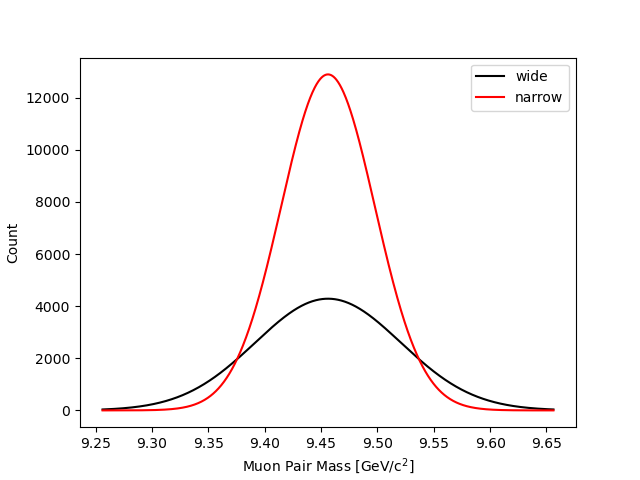
\includegraphics[width=0.7\columnwidth]{figures/double_gauss_test.png}
\caption{An example of the two Gaussian's that are summed in the double Gaussian fit. The double Gaussian consists of the wide Gaussian for the edge sections and the narrow Gaussian for the center.}
\label{fig:2d_hists_ex}
\end{figure}

This is useful when a peak is symmetric, with a tall, sharp middle section and a short, wide tail section. The quality of the fit was again determined by plotting a graph of residuals and calculating its 
reduced $\chi ^2$ value.

\addcontentsline{toc}{subsection}{Crystal Ball Fit}
\subsection*{Crystal Ball Fit}

The Crystal ball function was the most complex fit that we used on our data. It consists of two parts, an power-law tail on the low end and a Gaussian center region. The function itself is as follows:

\begin{equation}
        f(x)= N\cdot  
\begin{cases}
    a\cdot e^{-\frac{(x-\mu)^2}{2\cdot \sigma^2}},& \text{if } \frac{x-\mu}{\sigma}> -\alpha\\
    A\cdot (B-\frac{x-\mu}{\sigma})^{-n},    & \text{if } \frac{x-\mu}{\sigma}\leq -\alpha\\
\end{cases}
\end{equation}

Where, 

\begin{equation*}
    A = \left(\frac{n}{\lvert \alpha \rvert}\right)^{n}\cdot e^{(-\frac{\lvert \alpha \rvert^2}{2})}
\end{equation*}

\begin{equation*}
    B = \frac{n}{\lvert \alpha \rvert} - \lvert \alpha \rvert
\end{equation*}

\begin{equation*}
    N = \frac{1}{\sigma (C+D)}
\end{equation*}

\begin{equation*}
    C = \frac{n}{\lvert \alpha \rvert}\cdot \frac{1}{n-1}\cdot e^{(-\frac{\lvert \alpha \rvert^2}{2})}
\end{equation*}

\begin{equation*}
    D = \sqrt{\frac{\pi}{2}}\cdot \left(1+\text{erf}\left(\frac{\lvert \alpha \rvert}{\sqrt{2}}\right)\right)
\end{equation*}

And erf() is the error function. $N$ is a normalisation factor and $\alpha$, $n$, $\mu$ and $\sigma$ are the free parameters to be fitted. This function is often used to fit processes in high energy physics. The quality of this fit was also determined by plotting a graph of residuals and calculating its reduced $\chi ^2$ value. \\



\addcontentsline{toc}{section}{Results}
\section*{Results}

\addcontentsline{toc}{subsection}{Cleaning the Data}
\subsection*{Cleaning the Data}

Attempts at cleaning the data were made by neglecting terms outside of the
center regions on the Y-axis of 2D histogram plots of rapidity, transverse momentum of the muon pair, and the transverse momentum of each of
the individual muons against the invariant mass. The results of which were tested using the ratios method discussed in the methods section, showing that none of these showed any sign of cleaning the data, as both ratios were equal. This was to be expected, as none of the measured properties alone have any direct correlation to the origin of the signal. \\

The previously described cleaning method using the R-value was also implemented. First, the a graph showing the the correlation between the two muon pair momenta was plotted.

\begin{figure}[H]
\centering
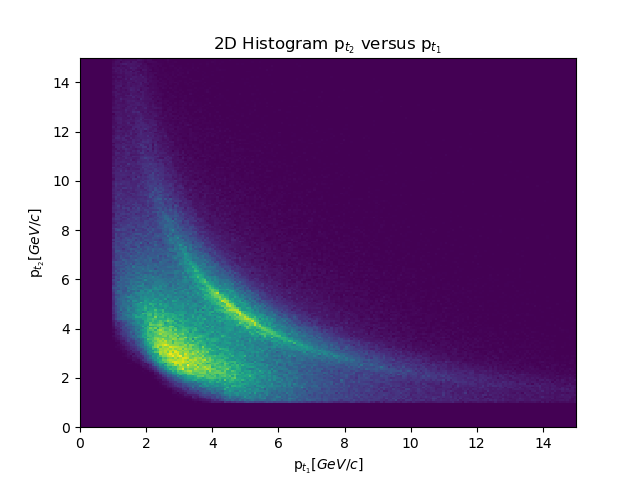
\includegraphics[width=0.7\columnwidth]{figures/mom_tran_1_2_2d_hist.png}
\caption{Graph of the transverse momenta of the two particles plotted against each other. Counts close to the 45$^o$ line are the counts of interest.}
\label{fig:2d_hists_ex}
\end{figure}

Values for R were calculated and plotted against the invariant muon pair mass.

\begin{figure}[H]
\centering
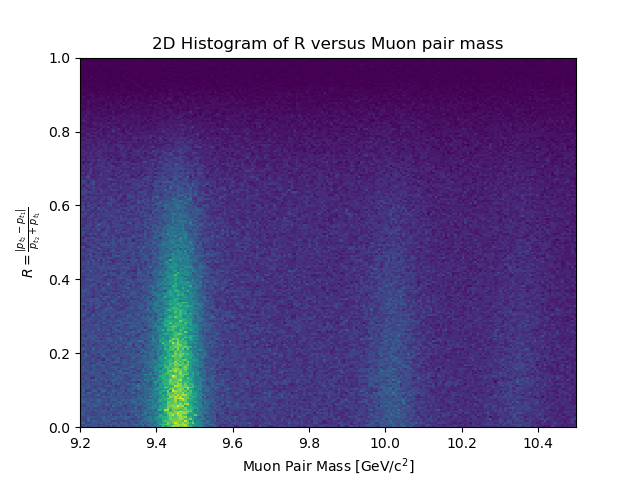
\includegraphics[width=0.7\columnwidth]{figures/xmass_sub_mom_tran_1_2_2d_hist.png}
\caption{R values against muon pair mass, showing the concentration of values at the peak region with low values of R, and relatively homogeneous counts in the background region.}
\label{fig:2d_hists_ex}
\end{figure}

From this, we made an initial estimation that a cutoff value of R=0.5 would be sufficient, however to be more rigorous, we decided to look at the spread of R values across the background regions and across the first peak region. The first peak region was used as this is the only peak that has sidebands that are unaffected by other peaks. 

\begin{figure}[H]
\centering
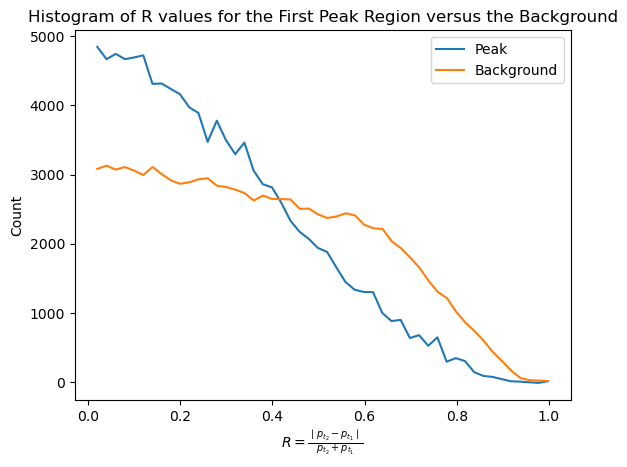
\includegraphics[width=0.6\columnwidth]{figures/r_val_graph.png}
\caption{Spread of R values across the first peak region and a background region, showing an obvious difference in shape of the curves.}
\label{fig:2d_hists_ex}
\end{figure}

This figure confirmed that the theory of the R value was successful in differentiating between signals from decays and background signals. Furthermore, the crossover point of roughly R=0.42 was taken to be a good cutoff value. So any signal with R$>$0.42 was discarded.\\

\begin{figure}[H]
\centering
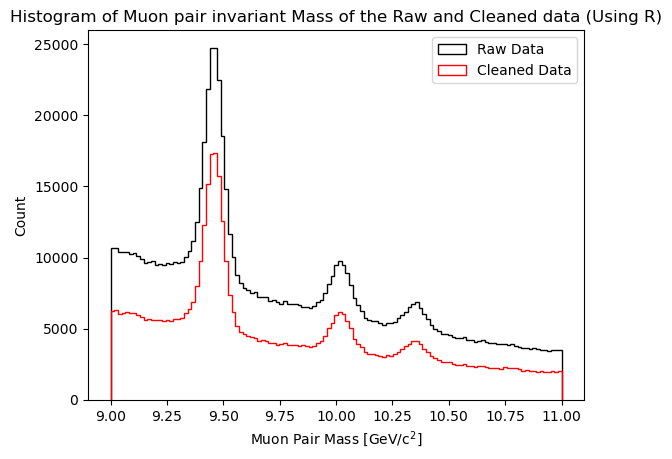
\includegraphics[width=0.6\columnwidth]{figures/cleaned_hist.png}
\caption{Histograms of the original data and the cleaned data}
\label{fig:2d_hists_ex}
\end{figure}

The resulting data was analysed by using the same ratios method. The results of which showed the background decreased by a factor of 1.705 whereas the peak region decreased by a factor of only 1.523, showing the data had been obviously cleaned. This cleaned data was then binned in a histogram and was used for the analysis in the report from this point onward.

\addcontentsline{toc}{subsection}{Exponential Background Fit}
% in the new method I m not actually taking the 
\subsection*{Exponential Background Fit}

The background regions were isolated and fitted with an exponential decay PDF (see equation (5)). The parameters of the PDF were
optimised using a negative log likelihood within PyRoot’s Fit() method.


\begin{figure}[H]
\centering
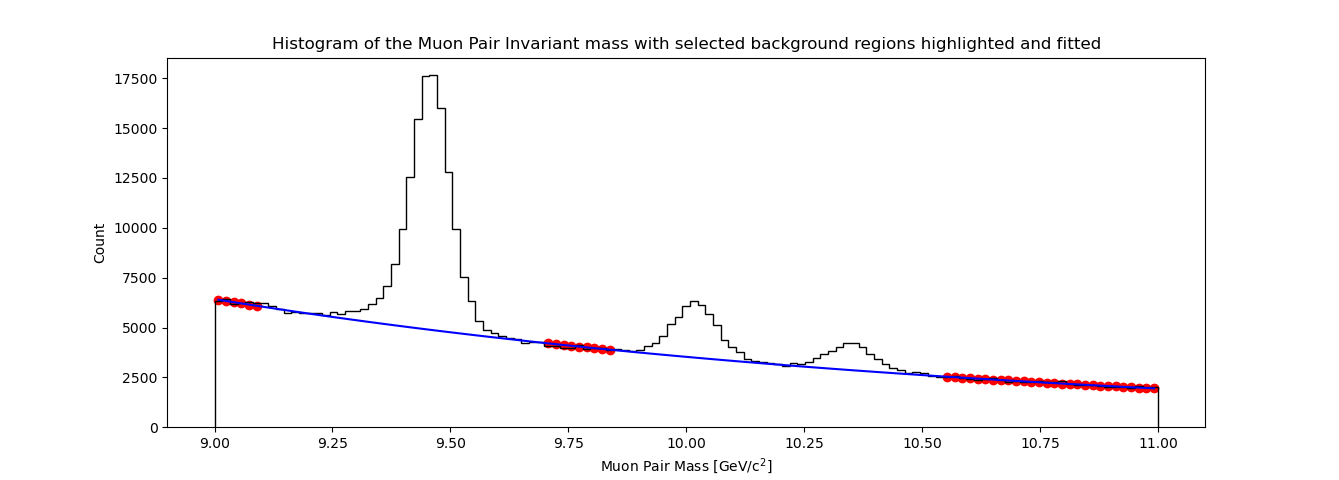
\includegraphics[width=0.9\columnwidth]{figures/expo_high_hist.png}
\caption{Histogram showing, in red, the points from which the exponential decay function was calculated. The fitted curve is also shown in blue.}
\label{fig:2d_hists_ex}
\end{figure}



\addcontentsline{toc}{subsection}{Gaussian Fit}
\subsection*{Gaussian Fit}

The PDF constructed to fit the data with Gaussian curves was the sum of three Gaussian's (equation 6) and an exponential decay (equation 5). All parameters of the PDF were optimised simultaneously using a negative log likelihood within PyRoot's \verb|Fit()| method.

\begin{figure}[H]
\centering
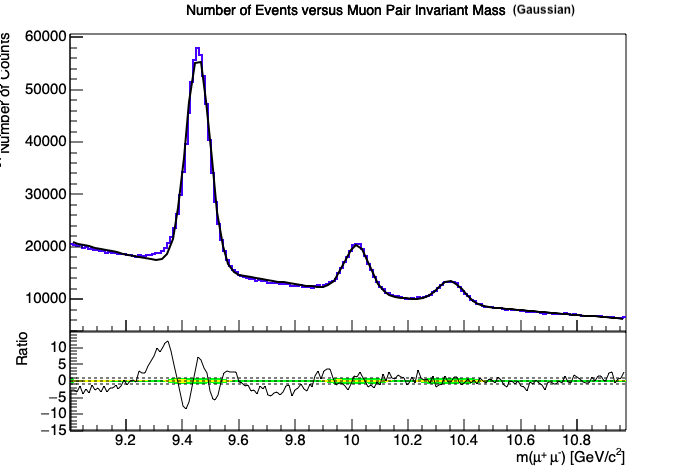
\includegraphics[width=0.7\columnwidth]{figures/xmass_hist_gauss.png}
\caption{Histogram showing the Gaussian curves fit to the three peaks, along with the exponential background fit.}
\label{fig:2d_hists_ex}
\end{figure}

Something to note about this graph is the excess of measurements on the low end of the first peak. The other models will attempt to rectify this discrepancy between the fit and the data. The reduced $\chi ^2$ was determined to be 9.976 for the single Gaussian fit.



\addcontentsline{toc}{subsection}{Double Gaussian Fit}
\subsection*{Double Gaussian Fit}

The PDF constructed to fit the peaks to Double Gaussian curves was the sum of three Double Gaussian's (equation 7) and an exponential decay (equation 5). All parameters of the PDF were optimised simultaneously using a negative log likelihood within PyRoot's \verb|Fit()| method. 

\begin{figure}[H]
\centering
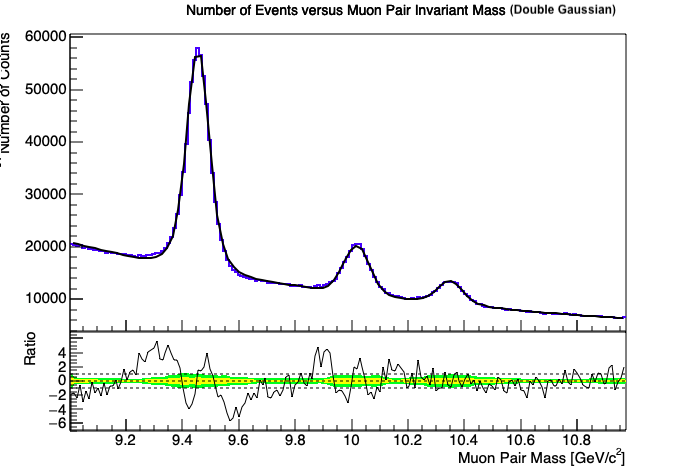
\includegraphics[width=0.7\columnwidth]{figures/xmass_hist_d_gauss.png}
\caption{Histogram showing the double Gaussian curves fit to the three peaks, along with the exponential background fit.}
\label{fig:2d_hists_ex}
\end{figure}

Although visually, the fit on the first peak is an obvious improvement from the single Gaussian, it is still limited by the fact that the fit is symmetric. The peaks(first peak especially) have long tails on the low end that a symmetric function cannot properly model. This is where the crystal ball function can be of use. This model's Reduced $\chi ^2$ value was found to be 4.791.

\addcontentsline{toc}{subsection}{Crystal Ball Fit}
\subsection*{Crystal Ball Fit}

The PDF constructed was the sum of three Crystal Ball's (equation 8) and an exponential decay (equation 5). All parameters of the PDF were optimised simultaneously using a negative log likelihood within PyRoot's \verb|Fit()| method.

\begin{figure}[H]
\centering
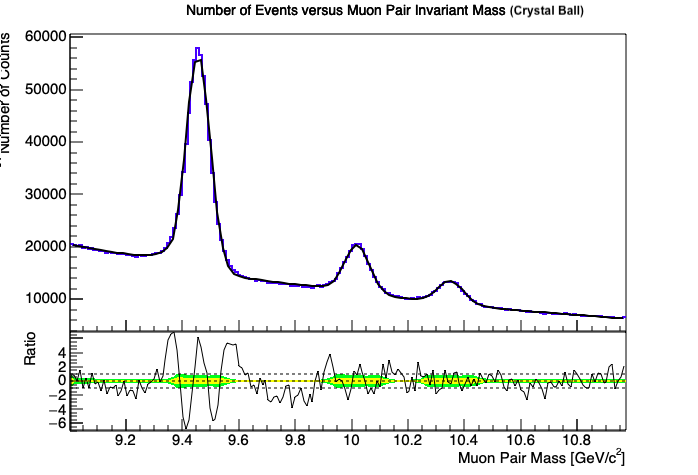
\includegraphics[width=0.7\columnwidth]{figures/xmass_hist_cb.png}
\caption{Histogram showing the crystal ball function curves fit to the three peaks, along with the exponential background fit.}
\label{fig:2d_hists_ex}
\end{figure}

 The values of \textalpha\ and $n$ are determined by fitting a Crystal Ball to the Monte-Carlo (MC) simulation data. These two parameters are then used to fit the actual data. The crystal ball fit resulted in a $\chi ^2$ value of 5.003.\\

\addcontentsline{toc}{section}{Discussion}
\section*{Discussion}
\addcontentsline{toc}{subsection}{Program Description}
\subsection*{Program Description}
Initially, all curve fitting was done using SciPy's \verb|curve_fit()| method, however this was unsuccessful in fitting the Crystal Ball (see figure 13 in appendix). The main issues arose when trying to fit the second and third peak. The normalisation of the Crystal Ball (see equation 6) depends on the values of \textalpha\ and n. It is likely that the Crystal Ball used, particularly the normalisation of this function, was not encoded properly leading to the incorrect fitting. \\

After failing at using SciPy, we tried fitting the binned data using Iminuit. Both our own function and ProbFit's inbuilt one's were tried and both of these methods proved unsuccessful at fitting a Crystal Ball to the MC data so they were not pursued further.\\

As a last ditched effort, we tried to use PyROOT and it's \verb|.Fit()|. As seen the Result section, all three models were successfully fitted to the binned data so PyRoot was used for the remainder of the analysis.\\

\addcontentsline{toc}{subsection}{Plot Analysis}
\subsection*{Plot Analysis}
The MC data was fitted with a Gaussian first to get initial guesses of amplitude, mean and standard deviation for the actual data (see figure 11). Then the MC data was fitted using PyRoot's inbuilt Crystal Ball to get values of \textalpha\ and n for the fit of the actual data (see figure 12). This was done because in the actual data, it is not possible to discriminate between the power law tail and the background. \\

The Muon Invariant Mass Pair data was then binned using the Freedman Diaconis method to determine the ideal bin width. The histogram was then fitted using 3 Probability Density functions:
\begin{enumerate}
    \item Sum of three Gaussian's and an exponential
    \item Sum of three double Gaussian's and an exponential
    \item Sum of three Crystal Ball's and an exponential
\end{enumerate}
For the Crystal Ball fit, the values of \textalpha\ and n were not allowed to vary and set to the values found when fitting the MC data.\\

The Gaussian PDF was especially unsuccessful a describing the asymmetry of the \textUpsilon(1s) peak as can be seen in the ratio plot on the lower end of the peak. The Gaussian also failed to properly describe the maxima of the \textUpsilon(1s) peak. The accuracy of the fit over the other peaks was greatly improved as can seen in the histogram and ratio plot.\\

The double Gaussian PDF was more successful than the single Gaussian in describing the data as a whole, especially the maxima of the \textUpsilon(1s) peak. However, it underestimated the low end and overestimated on the high end due to the symmetric nature of the function trying to describe asymmetric data. There was no visible improvement on the fit of the other two peaks.\\

The Crystal Ball PDF was significantly more successful than the Double Gaussian at dealing with the asymmetry of the \textUpsilon(1s) peak. The Crystal Ball PDF was also better at fitting the \textUpsilon(2s) peak as can be seen when comparing the ratio plot's of the double Gaussian and the Crystal Ball. However, its main shortcoming was in describing the amplitude of the \textUpsilon(1s) peak as can be seen in the ratio plot.\\

The reduced $\chi^2$ values of the different fitting models can be seen below:
\begin{table}[H]
\centering
\begin{tabular}{c|c}
Model           & Reduced $\chi^2$           \\ \hline
Gaussian        & 9.976 \\
Double Gaussian & 4.791 \\
Crystal Ball    & 5.003
\end{tabular}
\caption{Reduced \textchi$^2$ values for the different PDF's used to fit the binned data}
\label{tab:my-table}
\end{table}

When taking into account the residual analysis and \textchi$^2$ values in table 1, it was determined that the best PDF to describe the data was the double Gaussian. We will therefore use the Double Gaussian fit to calculate the masses of the \textUpsilon(1s), \textUpsilon(2s) and \textUpsilon(3s) mesons.

\addcontentsline{toc}{subsection}{Systematic Errors}
\subsection*{Errors}

The total error of our systems presented in the paper thus far have been estimated to comprise of 3 parts,

\begin{equation*}
    E_{tot} = \sqrt{E_{stat}^2 + E_{model}^2 + E_{back}^2}
\end{equation*}

$E_{stat}$ is simply the statistical error that is given by PyRoot's \verb|Fit()| function. $E_{model}$ is the systematic error that is given by our lack of knowledge in the data being correctly fitted by any of the functions that were tested. similarly, $E_{Back}$ is the systematic error in our background fit. These errors were estimated by looking at the differences in certain values of results obtained by the fits. So, in the models of the peaks, difference in the number of signal events obtained by the different fits can be compared. This difference can be expressed as a percentage and this percentage is taken to be the systematic error in the model of the peak. Similarly, for the background exponential fit, a good measure of the systematic uncertainty is to fit a linear equation (a polynomial could also be used) to the data, to which we can compare the exponential fit. A good way to compare these two fits would be to look at the area under the minimised curves. The difference in the number of signal events estimated by these two fits is again, a good gauge of the systematic error. From comparing all this data, we calculated the systematic error in the peak model to be $E_{model} =(1- \frac{4536}{4711})\cdot 100 = 3.7\%$ and the systematic error in the background model to be $E_{back} =(1- \frac{8815.088}{8815.111})\cdot 100 = 2.6\cdot 10^{-4}\%$. These errors are used to calculate the final errors in the values of the meson masses. \\

\addcontentsline{toc}{subsection}{Meson Masses}
\subsection*{Meson Masses}

Using the Double Gaussian fit, the masses of the three mesons and the total uncertainty in each of the values was calculated to be 9.4(3), 10.0(3) and 10.3(3) $[GeV/c^2]$.\\

\addcontentsline{toc}{section}{Conclusion}
\section*{Conclusion}
In conclusion the mass's of the \textUpsilon(1s), \textUpsilon(2s) and \textUpsilon(3s) mesons were determined to be 9.4(3), 10.0(3) and 10.3(3) $[GeV/c^2]$. The masses of the mesons were determined by binning the data using the Freedman Diaconis method and the resulting histogram was fitted using a Probability Density Function. This PDF was the sum of three double Gaussian's and an exponential decay. Of the different models that were tried, the double Gaussian was most successful in fitting the data overall, but was unable to correctly fit the asymmetry of the \textUpsilon(1s) peak. The fitting function that was able to best describe the asymmetry was the Crystal Ball, but it fell short when fitting the amplitude of the \textUpsilon(1s) peak. The errors were determined by combining statistical errors and systematic errors. For future work, one could fit the histogram using double Crystal Ball functions instead of the single Crystal Ball's. This was not done due to a lack of time.
\newpage
\addcontentsline{toc}{section}{Appendix}
\section*{Appendices}
The github repository for the project can be found \href{https://github.com/aqnemo32/project_f1_dah}{by clicking here}.
\begin{figure}[H]
    \centering
    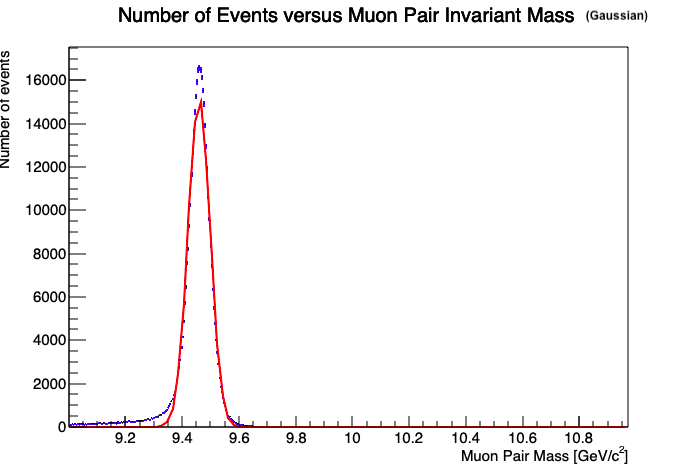
\includegraphics[width = 0.7\textwidth]{figures/xmass_mc_gauss_hist.png}
    \caption{MC Data Histogram fitted using a single Gaussian function}
    \label{fig:my_label}
\end{figure}
\begin{figure}[H]
    \centering
    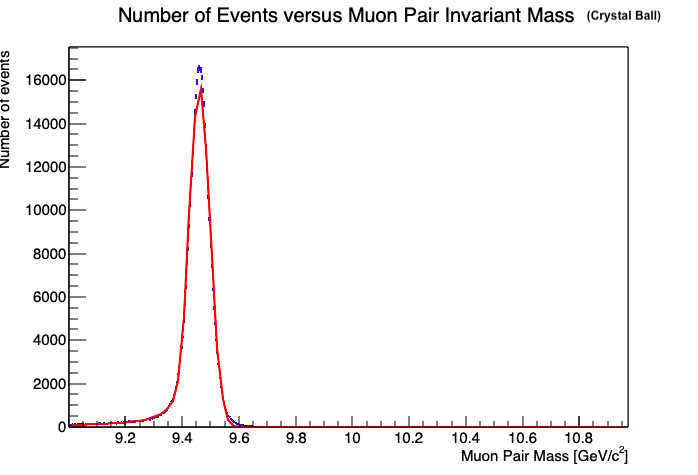
\includegraphics[width = 0.7\textwidth]{figures/xmass_mc_hist_cb.png}
    \caption{MC Data Histogram fitted using a Crystal Ball function, \textalpha\ = 1.809(9) n = 1.21(7)}
    \label{fig:my_label}
\end{figure}
\begin{table}[H]
\centering
\begin{tabular}{c|c|c|c|c}
Name          & Value        & Error       & Step Size    & First Derivative \\ \hline
1 A           & 4.02667e+04  & 1.02082e+02 & 2.25030e-02  & 5.76845e-08      \\
1 \textmu\    & 9.45584e+00  & 1.07103e-04 & -5.33873e-09 & -2.71954e-02     \\
1 \textsigma\ & 4.30333e-02  & 1.06615e-04 & 3.69184e-08  & 1.80417e-01      \\
2 A           & 9.05194e+03  & 6.21961e+01 & 1.24387e-02  & 1.80123e-07      \\
2 \textmu\    & 1.00190e+01  & 3.21421e-04 & 1.05159e-07  & -2.55114e-02     \\
2 \textsigma\ & 4.46576e-02  & 3.34852e-04 & 1.23332e-08  & 3.47965e-02      \\
3 A           & 4.23485e+03  & 5.04731e+01 & 4.89402e-03  & -1.43702e-07     \\
3 \textmu\    & 1.03499e+01  & 5.90210e-04 & 2.40900e-08  & -7.31417e-02     \\
3 \textsigma\ & -4.64171e-02 & 6.25562e-04 & -1.70275e-07 & -2.77189e-03     \\
\textdelta\   & 8.48441e+00  & 6.78182e-03 & 3.34106e-06  & 1.38454e-02      \\
c             & -6.08244e-01 & 1.30511e-03 & -5.96469e-07 & 9.52061e-02      \\
A             & 1.03813e+03  & 6.25971e+00 & 3.11688e-03  & 1.31380e-05     
\end{tabular}
\caption{Results generated by PyRoot's \lstinline{Fit()} method for the single Gaussian PDF}
\label{tab:my-table}
\end{table}

\begin{table}[H]
\centering
\begin{tabular}{c|c|c|c|c}
Name            & Value        & Error       & Step Size    & First Derivative \\ \hline
1 A           & 4.19031e+04  & 1.22585e+02 & -8.31575e-02 & -1.22436e-06     \\
1 \textmu\      & 9.45592e+00  & 1.04640e-04 & -2.28874e-08 & -3.07035e-01     \\
1 \textsigma\ 1 & 3.59877e-02  & 4.30320e-04 & -1.97417e-08 & -7.89929e-01     \\
1 \textsigma\ 2 & 6.78501e-02  & 1.74680e-03 & 2.85243e-07  & 4.89407e-01      \\
1 b             & 7.72830e-01  & 1.96890e-02 & 1.02867e-05  & -3.51944e-03     \\
2 A            & 1.07839e+04  & 6.94048e+01 & 6.99406e-02  & -1.81525e-05     \\
2 \textmu\      & 1.00187e+01  & 3.24829e-04 & -9.00187e-08 & -9.08082e-01     \\
2 \textsigma\ 1 & 4.62946e-02  & 3.58171e-04 & -4.13757e-07 & -2.28467e+00     \\
2 \textsigma\ 2 & 1.59859e+01  & 3.02043e+00 & 6.88108e-03  & -2.35227e-02     \\
2 b             & 8.50324e-01  & 2.41709e-03 & -6.26180e-06 & 1.51863e-01      \\
3 A           & 4.41384e+03  & 5.72334e+01 & 7.88747e-02  & -4.26049e-06     \\
3 \textmu\      & 1.03495e+01  & 6.05410e-04 & 1.83102e-07  & -7.83342e-02     \\
3 \textsigma\ 1 & 4.31168e-02  & 1.29983e-03 & -8.54064e-07 & -4.68366e-01     \\
3 \textsigma\ 2 & 9.98015e-02  & 1.28481e-02 & -2.99539e-05 & -1.99121e-01     \\
3 b             & 8.76737e-01  & 3.84768e-02 & -2.67342e-04 & 3.07646e-02      \\
\textdelta\     & 8.65497e+00  & 4.02109e-02 & 9.56470e-05  & -5.49157e-01     \\
c               & -6.78884e-01 & 8.79190e-03 & -2.05141e-05 & -1.28723e+01     \\
A               & 1.53534e+03  & 5.51426e+01 & 1.30764e-01  & -3.57758e-04    
\end{tabular}
\caption{Results generated by PyRoot's \lstinline{Fit()} method for the Double Gaussian PDF}
\label{tab:my-table}
\end{table}

\begin{table}[H]
\centering
\begin{tabular}{c|c|c|c|c}
Name            & Value        & Error       & Step Size    & First Derivative \\ \hline
1 A              & 4.09813e+04  & 1.04094e+02 & -2.08780e-02 & 4.37847e-07      \\
1 \textmu\      & 9.45620e+00  & 1.05680e-04 & 4.81710e-08  & 8.06710e-02      \\
1 \textsigma\   & 4.28614e-02  & 1.10387e-04 & 1.91373e-08  & 7.34546e-01      \\
1 \textalpha\ & 1.80980e+00  & fixed       & 2.85243e-07  & 4.89407e-01      \\
1 n              & 1.21473e+00  & fixed       & 1.02867e-05  & -3.51944e-03     \\
2 A             & 9.22557e+03  & 6.33284e+01 & -2.02218e-02 & -1.05139e-08     \\
2 \textmu\     & 1.00190e+01  & 3.21474e-04 & 1.81114e-07  & 6.76821e-02      \\
2 \textsigma\    & 4.47205e-02  & 3.44729e-04 & 7.19397e-08  & 1.24630e-01      \\
2 \textalpha\   & 1.80980e+00  & fixed       & 6.88108e-03  & -2.35227e-02     \\
2 n              & 1.21473e+00  & fixed       & -6.26180e-06 & 1.51863e-01      \\
3 A             & 4.31683e+03  & 5.05537e+01 & -1.32157e-02 & -9.62037e-08     \\
3 \textmu\       & 1.03498e+01  & 5.92742e-04 & 2.20053e-07  & 1.83512e-02      \\
3 \textsigma\    & 4.72744e-02  & 6.39671e-04 & 7.50086e-08  & 2.52552e-02      \\
3 \textalpha\  & 1.80980e+00  & fixed       & -2.99539e-05 & -1.99121e-01     \\
3 n             & 1.21473e+00  & fixed       & -2.67342e-04 & 3.07646e-02      \\
\textdelta\     & 8.32579e+00  & 6.82188e-03 & 6.10146e-06  & 5.81992e-02      \\
c               & -5.83207e-01 & 1.34918e-03 & -1.13859e-06 & 5.56388e-01      \\
A               & 9.30118e+02  & 6.01620e+00 & 5.38628e-03  & 6.24777e-05     
\end{tabular}
\caption{Results generated by PyRoot's \lstinline{Fit()} method for the Crystal Ball PDF}
\label{tab:my-table}
\end{table}

\begin{figure}[H]
    \centering
    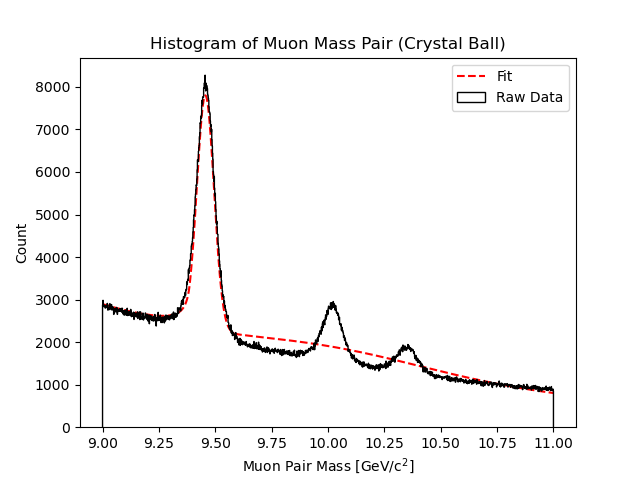
\includegraphics{figures/cb_hist.png}
    \caption{Crystal Ball PDF fit to Mass histogram using SciPy's \lstinline{curve_fit()}. The fitting clearly fails to properly fit the second and third peak. This was caused by the normalisation of the Crystal Ball being wrong.}
    \label{fig:my_label}
\end{figure}

\bibliographystyle{unsrt}
\bibliography{refs.bib}

\end{document}
